\section{Architecture}

L'architecture du code de notre projet se présente sous forme de diagramme dans lequelle on retrouve dans un premier temps deux sections sginificatives : une qui concerne les infrastructures avec les constructions humaines tel que les routes, les bâtiments, et la muraille; et une autre qui concerne le terrain et les éléments environnementaux qui le compose comme les arbres, l'herbe etc..

\begin{center}
    \centering
    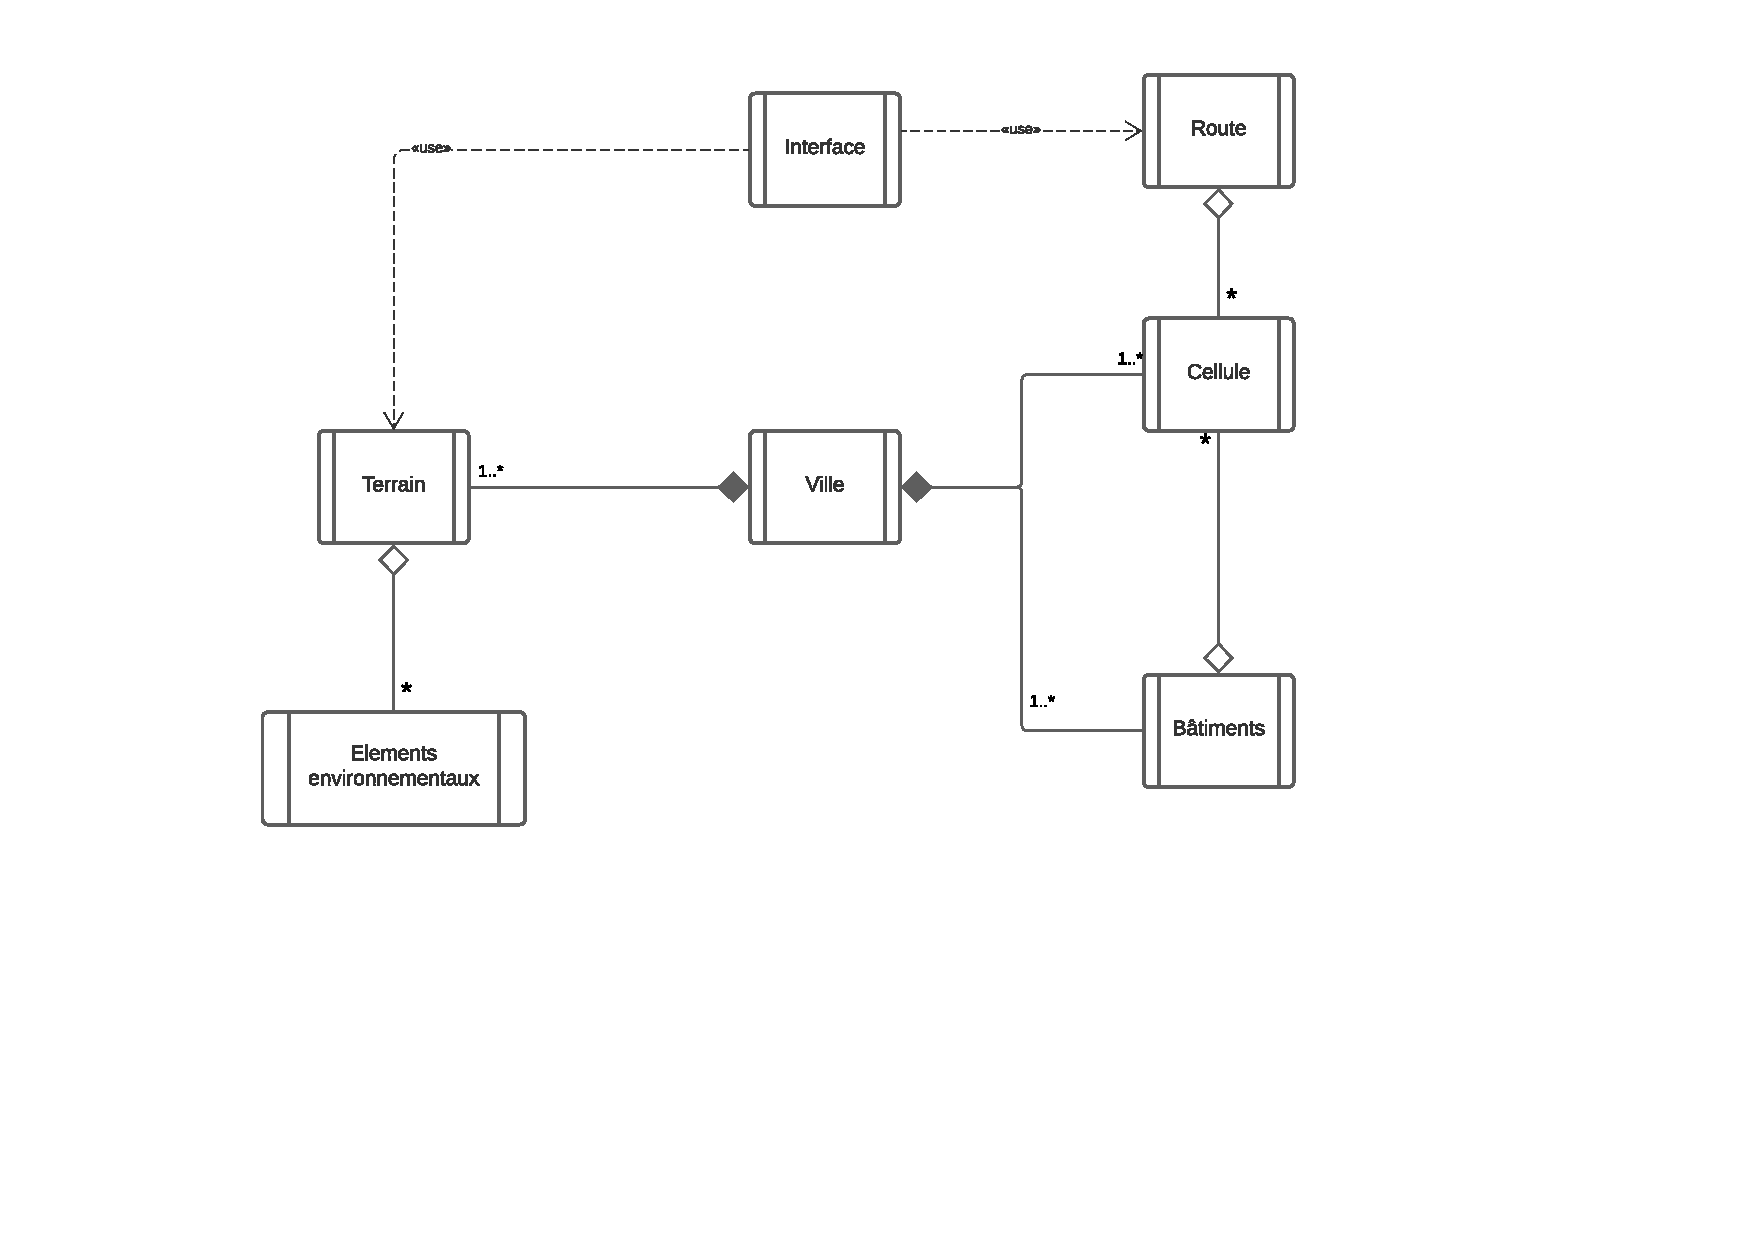
\includegraphics[height = 8 cm]{images/DiagrammeSimple.pdf}\\
\end{center}

Il existe également une autre version de notre architecture qui cette fois-ci est beaucoup plus précise puisqu'elle se compose des classes principales de notre code à savoir :
\begin{itemize}
	\item Générer une ville qui va faire appel à générer un terrain, des bâtiments, des routes et des cellules.
	\item Le terrain qui va générer une surface en relief grâce au bruit de Perlin, des rivières et de la végétation comme des arbres et de l'herbe.
	\item Les bâtiments qui vont être générés par type de bâtiment et sur des cellules dans lesquelles on va également générer les routes.
	\item Une interface utilisateur qui met en place des informations comme générer le nombre de bâtiments, de routes, etc..
\end{itemize}

\begin{center}
    \centering
    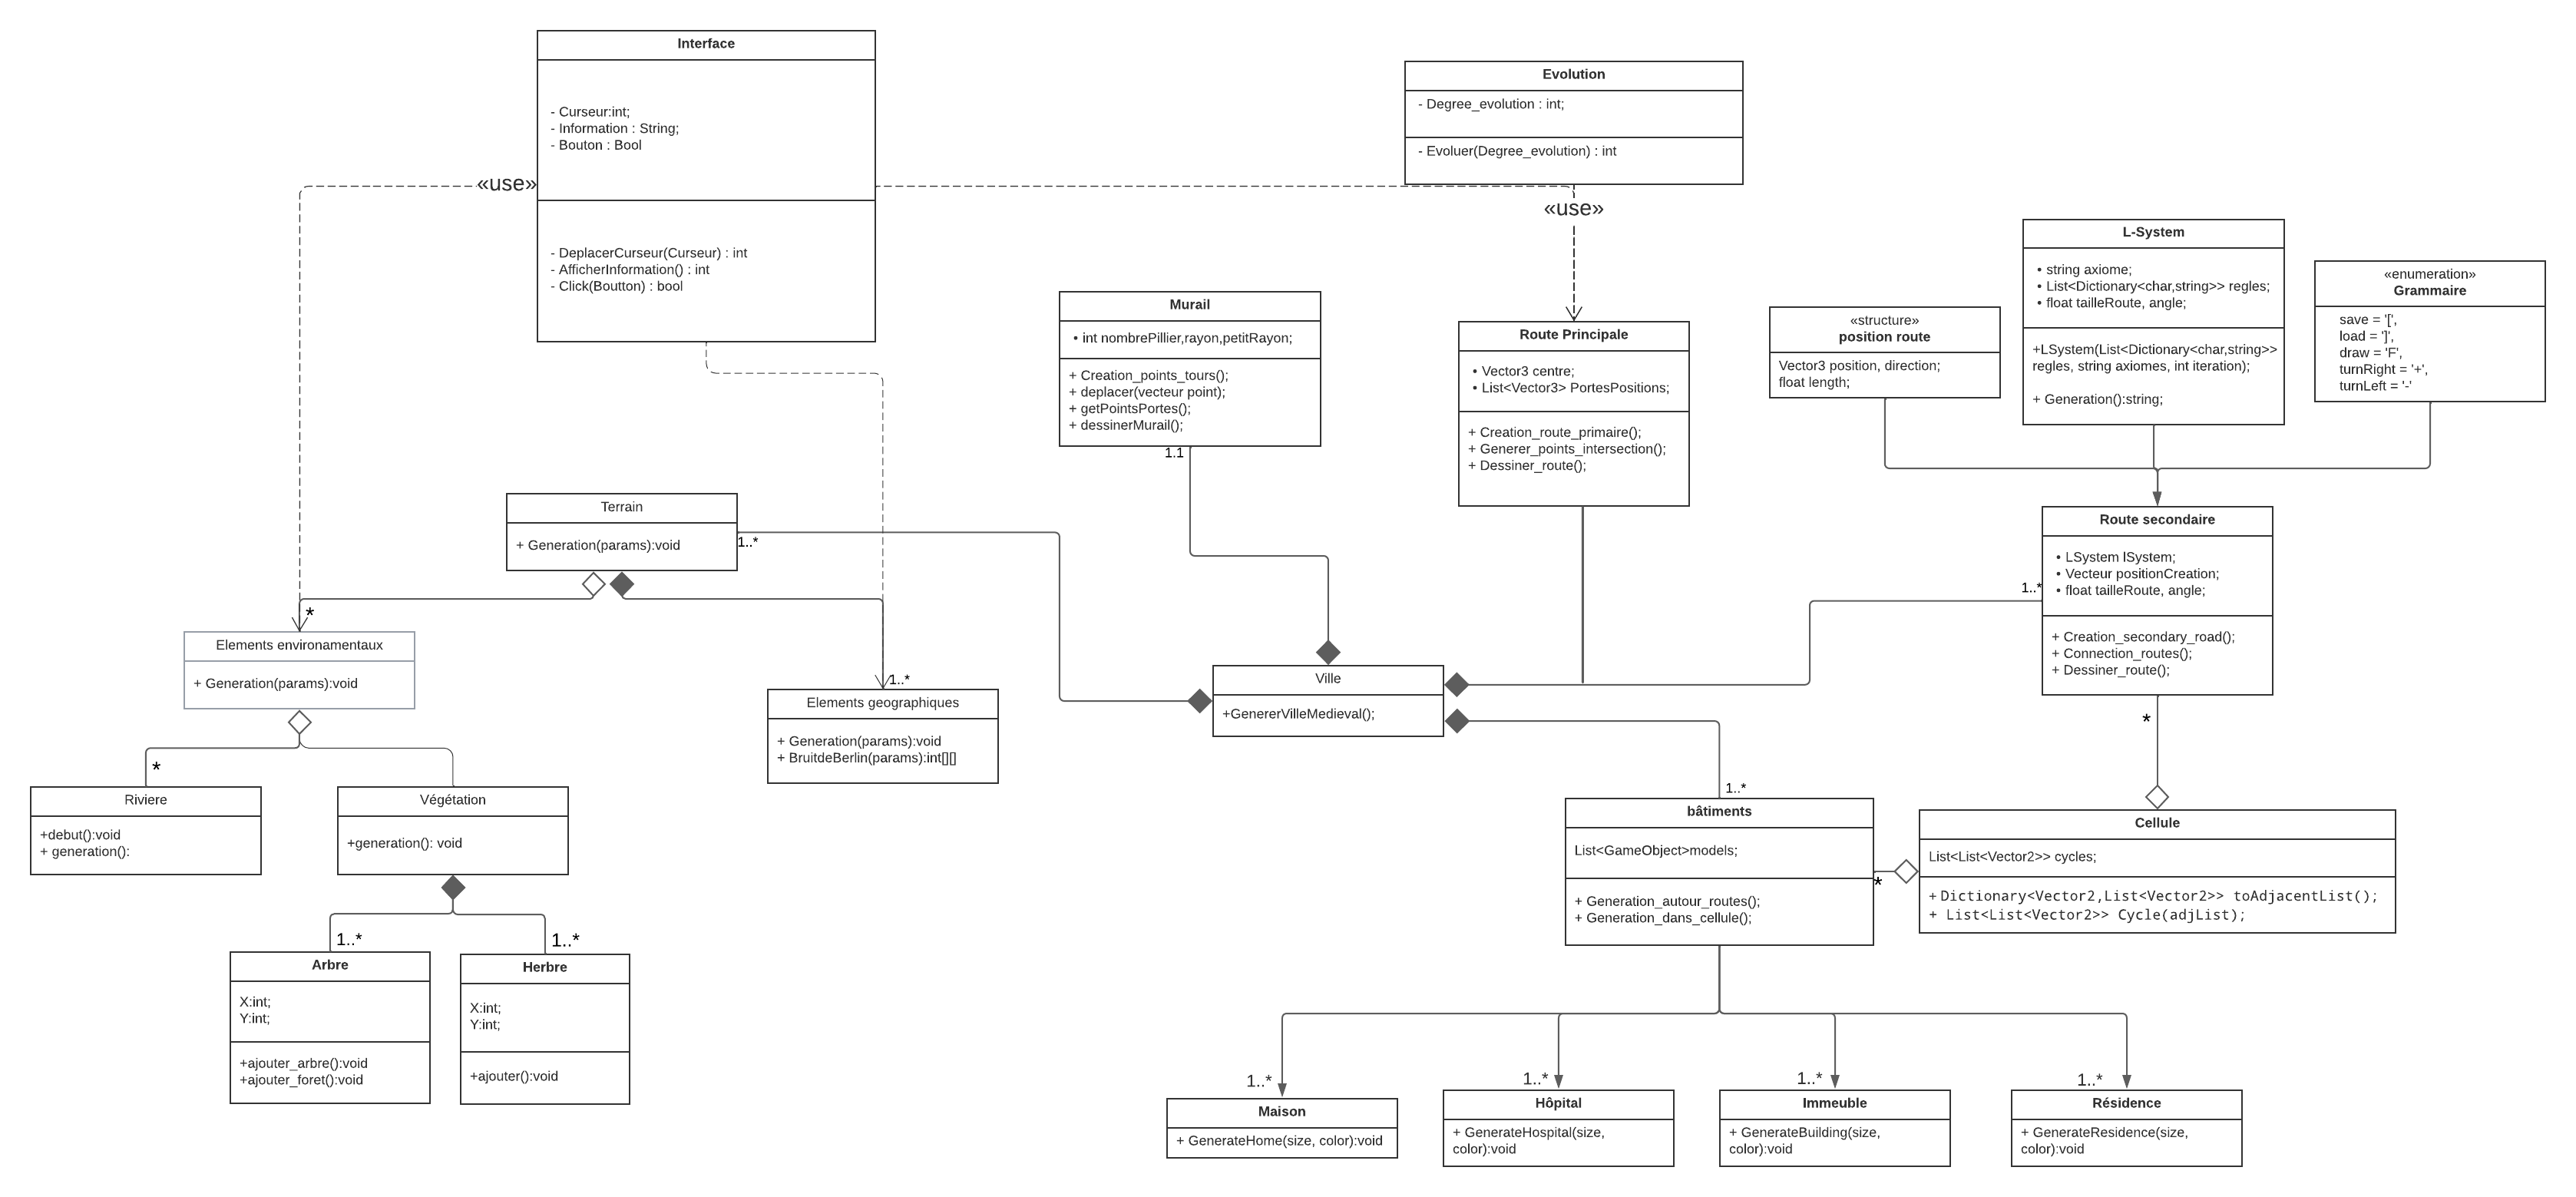
\includegraphics[height = 13 cm, angle = 90]{images/Diagramme_V5.png}\\
\end{center}